\section{Stand der Technik}
\autor{Medjen Izairi}
Für die Gestaltung und Anpassung der Behavior Tree in unserem Projekt verwenden wir Groot2, als eine fortschrittliche Software, die sich durch ihre benutzerfreundliche Drag-and-Drop-Oberfläche auszeichnet. Diese intuitive Benutzeroberfläche ermöglicht es Benutzern, Behavior Trees mühelos zu erstellen und zu bearbeiten, indem sie Knoten per Drag-and-Drop hinzufügen, verschieben und miteinander verbinden können.
Die Software erleichtert zudem die effiziente Verwaltung von umfangreichen Projekten durch die Unterstützung mehrerer Dateien. Diese Funktion ermöglicht es, den Überblick über komplexe Systeme zu behalten und die Arbeit an großen Verhaltensbaumprojekten zu optimieren.
\cite{groot2}\\

Eine weitere herausragende Funktion von Groot2 ist die Echtzeitvorschau des generierten XML-Codes des Behavior Trees. Die Funktion bietet einen klaren Überblick über die zugrunde liegende Struktur des Baums, wodurch die Entwicklungs- und Debugging-Prozesse optimiert werden. Insgesamt bietet Groot2 eine vielseitige und leistungsfähige Umgebung für die Entwicklung und Verwaltung von Behavior Tree, die sich durch Benutzerfreundlichkeit, Kompatibilität und erweiterte Funktionen auszeichnet.\cite{groot2}

\begin{figure}[H]
    \centering
    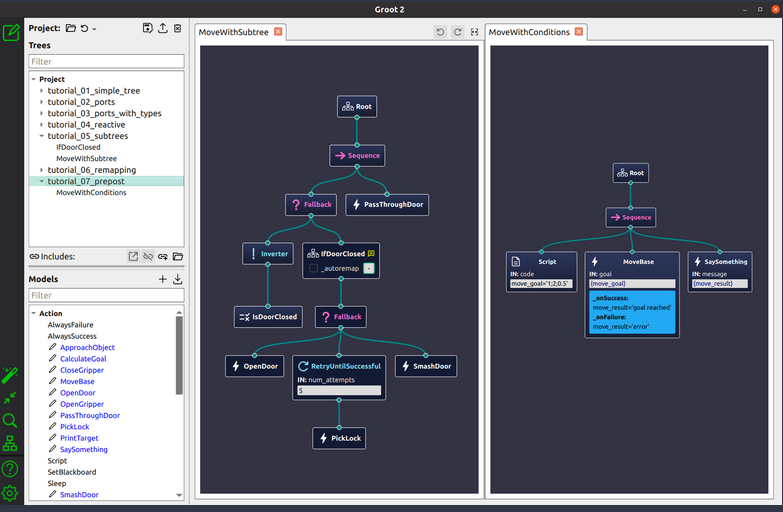
\includegraphics[width=0.85\linewidth]{Pictures/grafik2_groot2.png}
    \caption{Groot2}
    \cite{groot2}
\end{figure}

